

\documentclass[11pt,notitlepage]{article}

%\documentclass[twocolumn,secnumarabic,amssymb, nobibnotes, aps, prd]{revtex4-1}
%\documentclass[aps,preprint]{revtex4}
%\documentclass[pra,preprint]{revtex4}
%\documentclass[pra,twocolumn]{revtex4}

\usepackage[lmargin=1.in,rmargin=1.in,tmargin=1.in,bmargin=1in]{geometry}
\usepackage{setspace} %\doublespacing
\usepackage[pdftex]{graphicx}
\usepackage{subfig}
\usepackage{latexsym}
\usepackage{amsfonts}
\usepackage{amsmath,revsymb,graphicx} 
\usepackage{natbib}
\usepackage{longtable}
\usepackage{titling}
\usepackage[
	pdfauthor={Brian Weinstein},
	pdftitle={The Association Between Felonies in NYC and Weather and Temporal Conditions},
	bookmarks=true,
	colorlinks=true,
	linkcolor=blue,
	urlcolor=blue,
	citecolor=blue,
	pdftex,
	linktocpage=true
	]{hyperref}
\usepackage[textsize=tiny]{todonotes}
\usepackage{authblk}
\usepackage{float}
\usepackage{caption}
\usepackage{xspace}
\usepackage{underscore} % can't use underscores in file names (e.g., image names) when using this package
%\usepackage{enumitem} \setlist{nosep}


\usepackage{xcolor}
\usepackage{adjustbox}
\usepackage{verbatim}
\definecolor{shadecolor}{rgb}{.9, .9, .9}
\newenvironment{codeSmall}%
   {\par\noindent\adjustbox{margin=1ex,bgcolor=shadecolor,margin=0ex \medskipamount}\bgroup\minipage\linewidth\verbatim\footnotesize}%
   {\endverbatim\endminipage\egroup}


\newcommand{\degf}{^\circ\text{F}}




\begin{document}

\title{The Association Between Felonies in NYC and Weather and Temporal Conditions}
\author{Brian Weinstein}
\affil{\textit{Columbia University} \\ \textit{STAT W4201: Advanced Data Analysis}}
\date{May 2, 2016}

\maketitle



\begin{abstract}
\singlespacing

\todo{UPDATE THE ABSTRACT}

\noindent \textbf{Background:} The New York City Police Department recently released incident-level felony data to the New York City Open Data portal. The dataset includes timestamped information for all felonies committed in NYC.

We first examine the association between the daily number of felonies committed in NYC in 2015 and temperature, presence of precipitation, day of week, federal and New York holidays, and school days. Second, we examine the association between changes in the number of felonies (as compared to the previous day) and large increases in temperature ($>8 \degf$ from the previous day).

\noindent \textbf{Methods and Results:} We initially test for a difference between the number of felonies on warmer and cooler days ($\geq 51.98 \degf$ and $< 51.98 \degf$, respectively --- the NYC 2015 median), finding overwhelming evidence of a difference, with there being 44 more felonies, on average, on warmer days than on cooler day (95\% CI 38 to 51 felonies; two sided p-value $<0.000001$ from a two-sample t-test). \todo{Remove this.}

After accounting for presence of precipitation, holidays, school days, and day of week, the data provides overwhelming evidence that for every $1 \degf$ increase in temperature there are, on average, 1.4 additional felonies per day (95\% CI 1.3 to 1.6 felonies; two-sided p-value $<0.000001$ for a test that the linear regression coefficient is 0). \todo{Explain that the results change after removing observations with large studentized residuals.}

We next find that, after accounting for day of week, there is little evidence to suggest that increases in felonies from the previous day are associated with large increases in temperature (two-sided p-value 0.1001 for a test that the linear regression coefficient is 0).

\noindent \textbf{Conclusions:} There is a clear association between warmer temperatures and an increased number of felonies. There is no evidence that large increases in temperature from the previous day are associated with increases in the number of felonies.




\end{abstract}



\pagebreak

\singlespacing



\section{Introduction}



After many years of pressure, the New York City Police Department (NYPD) recently released incident-level felony data to the NYC Open Data portal, as part of their initiative to improve their accessibility, transparency, and accountability. Prior to this release, felony data had only been provided in an aggregated format (by week and police precinct), and was done so only in PDF and Excel files on a weekly and quarterly basis.

In this paper, we use the newly-released data to examine the association between the daily number of felonies committed in New York City (NYC) and: day of week, outside air temperature, precipitation, federal and New York (NY) holidays, and public school days.

\subsection{Questions of Interest}

In this paper we study three main questions of interest:

\begin{enumerate}
\setlength\itemsep{-1pt}
\item Are felonies associated with temperature? After taking temperature into account, is felonies associated with precipitation, school days, holidays, and day of week?
\item Although there’s no causal relationship, for a given set of these conditions, how many felonies can the NYPD reasonably expect?
\item Are changes in the number of felonies, as compared to the previous day, associated with large ($>8 \degf$) increases in temperature, after taking into account temperature, precipitation, school days, holidays, and day of week?
\end{enumerate}



\subsection{Dataset}
\label{sec:dataset}

The class, description, and source for each variable in the dataset is outlined below. Only those variables used in the analyses are included here --- redundant and untranformed variables that were removed during exploratory analysis are not described below. The dataset contains 365 observations, one for each date in 2015.

\begin{itemize}
\setlength\itemsep{-1pt}

\item \texttt{felonies} (integer) is a count of the number of felonies committed on each day in NYC in 2015. The values are derived counts from the ``NYPD 7 Major Felony Incidents'' dataset in the NYC Open Data Portal [\href{https://data.cityofnewyork.us/Public-Safety/NYPD-7-Major-Felony-Incidents/hyij-8hr7}{data.cityofnewyork.us/d/hyij-8hr7}]. The felonies included in the dataset that contribute to the overall daily count are burglary, felony assault, grand larceny, grand larceny of motor vehicle, murder and non-negligent manslaughter, rape, and robbery.

\item \texttt{temp_min_degF} (numeric) is the minimum daily temperature on the given date (in degrees Fahrenheit), as reported by the New York Central Park Belvedere Tower weather station. The data was requested via the National Centers for Environmental Information [\href{http://www.ncdc.noaa.gov/cdo-web/search}{ncdc.noaa.gov/cdo-web/search}].

\item \texttt{is_warm} (factor) is an indicator variable, taking value ``1'' if \texttt{temp_min_degF} is $\geq 51.98 \degf$ (the median for 2015) on the given date, and ``0'' otherwise.

\item \texttt{any_precip} (factor) is an indicator variable, taking value ``1'' if there was any precipitation on the given date, and ``0'' otherwise. See \texttt{temp_min_degF} for source information.


\item \texttt{is_holiday} (factor) is an indicator variable, taking value ``1'' if the given date is a NY or federal holiday, or value ``0'' otherwise. The NY and federal holidays were defined using the lists provided by the NY State Department of Civil Service [\href{https://www.cs.ny.gov/attendance_leave/2015_legal_holidays.cfm}{cs.ny.gov/attendance_leave/2015_legal_holidays.cfm}] and U.S. Office of Personnel Management [\href{https://www.opm.gov/policy-data-oversight/snow-dismissal-procedures/federal-holidays/\#url=2015}{opm.gov/policy-data-oversight/snow-dismissal-procedures/federal-holidays/\#url=2015}], respectively.


\item \texttt{is_school_day} (factor) is an indicator variable, taking value ``1'' if NYC Public Schools were open and in session on the given date, or value ``0'' otherwise. Although the NYC Department of Education publishes this data to the NYC Open Data Portal, the historical data is only retained there for the current school year. Instead we scrape the attendance data from XML files in Aaron Schumacher's ``NYCattends'' Github repository [\href{https://github.com/ajschumacher/NYCattends/tree/master/xml}{github.com/ajschumacher/NYCattends/tree/master/xml}].
% link in the NYC Open Data Portal: \href{https://data.cityofnewyork.us/Education/Attendance-4PM-Report/madj-gkhr}{data.cityofnewyork.us/d/madj-gkhr}


\item \texttt{day_of_week} (factor) is a categorical variable indicating the day of week (Sunday=``1'', Monday=``2'' $, \ldots, $ Saturday=``7''). 

\item \texttt{felonies_diff} (numeric) indicates for a given date the difference in the number of felonies as compared to the previous day. On Jan. 3, 2015, for example, \texttt{felonies_diff} = 6, since there were 6 more felonies committed on Jan. 3 than on Jan. 2.

\item \texttt{temp_min_degF_diff} (numeric) indicates for a given date the difference in \texttt{temp_min_degF} as compared to the previous day. On Jan. 3, 2015, for example, \texttt{temp_min_degF_diff} = -1.98, since the daily minimum temperature (\texttt{temp_min_degF}) was $1.98 \degf$ lower on Jan. 3 than on Jan. 2.

\item \texttt{temp_jump} (factor) is an indicator variable, taking value ``1'' if \texttt{temp_min_degF_diff} $> 8$, or value ``0'' otherwise. An increase of $> 8 \degf$ puts the day of interest in the top 10\% of temperature increases in 2015.

\end{itemize}

%\begin{center}
%    \begin{tabular}{ | l | l | p{5cm} | p{5cm} |}
%    \hline
%    Variable Name & Class & Description & Source \\ \hline \hline
%    \texttt{date} & Date & Date of observation. &  \\ \hline
%    \texttt{felonies} & Numeric & Number of felonies occurring on the indicated date. & Cloudy with rain, across many northern regions. Clear spells 
%    across most of Scotland and Northern Ireland, 
%    but rain reaching the far northwest. \\ \hline
%    Wednesday & 10C & 21C & Rain will still linger for the morning. 
%    Conditions will improve by early afternoon and continue 
%    throughout the evening. \\
%    \hline
%    \end{tabular}
%\end{center}

\subsection{Report Overview}

In Section \ref{sec:eda} we present some exploratory analysis and plots, in Sections \ref{sec:linearRegressionModelAndAssumptions} and \ref{sec:statisticalAnalysisAndInference} we walkthrough the model setup and statistical analysis, in Section \ref{sec:modelChecking} we do some model checking, and in Section \ref{sec:conclusion} we present our conclusions. \todo{update this}



\section{Exploratory Analysis and Data Cleaning}
\label{sec:eda}

We first examine pairwise scatterplots of some of the numeric variables in the raw dataset (\texttt{felonies}, \texttt{temp_min_degF}, \texttt{temp_max_degF}, and \texttt{school_attendance_pct}), as shown in Figure \ref{fig:pairsNumericExclAcc}. From this figure we first notice that there are approximately linear relationships between \texttt{felonies} and \texttt{temp_min_degF}, and between \texttt{felonies} and \texttt{temp_max_degF}. There is also strong collinearity between \texttt{temp_min_degF} and \texttt{temp_max_degF} (correlation: 0.969), however, so we remove one of these variables (\texttt{temp_max_degF}) from the covariates that will be used in the regression model.

\begin{figure}[!h]
	\centering
	\captionsetup{width=0.9\textwidth}
	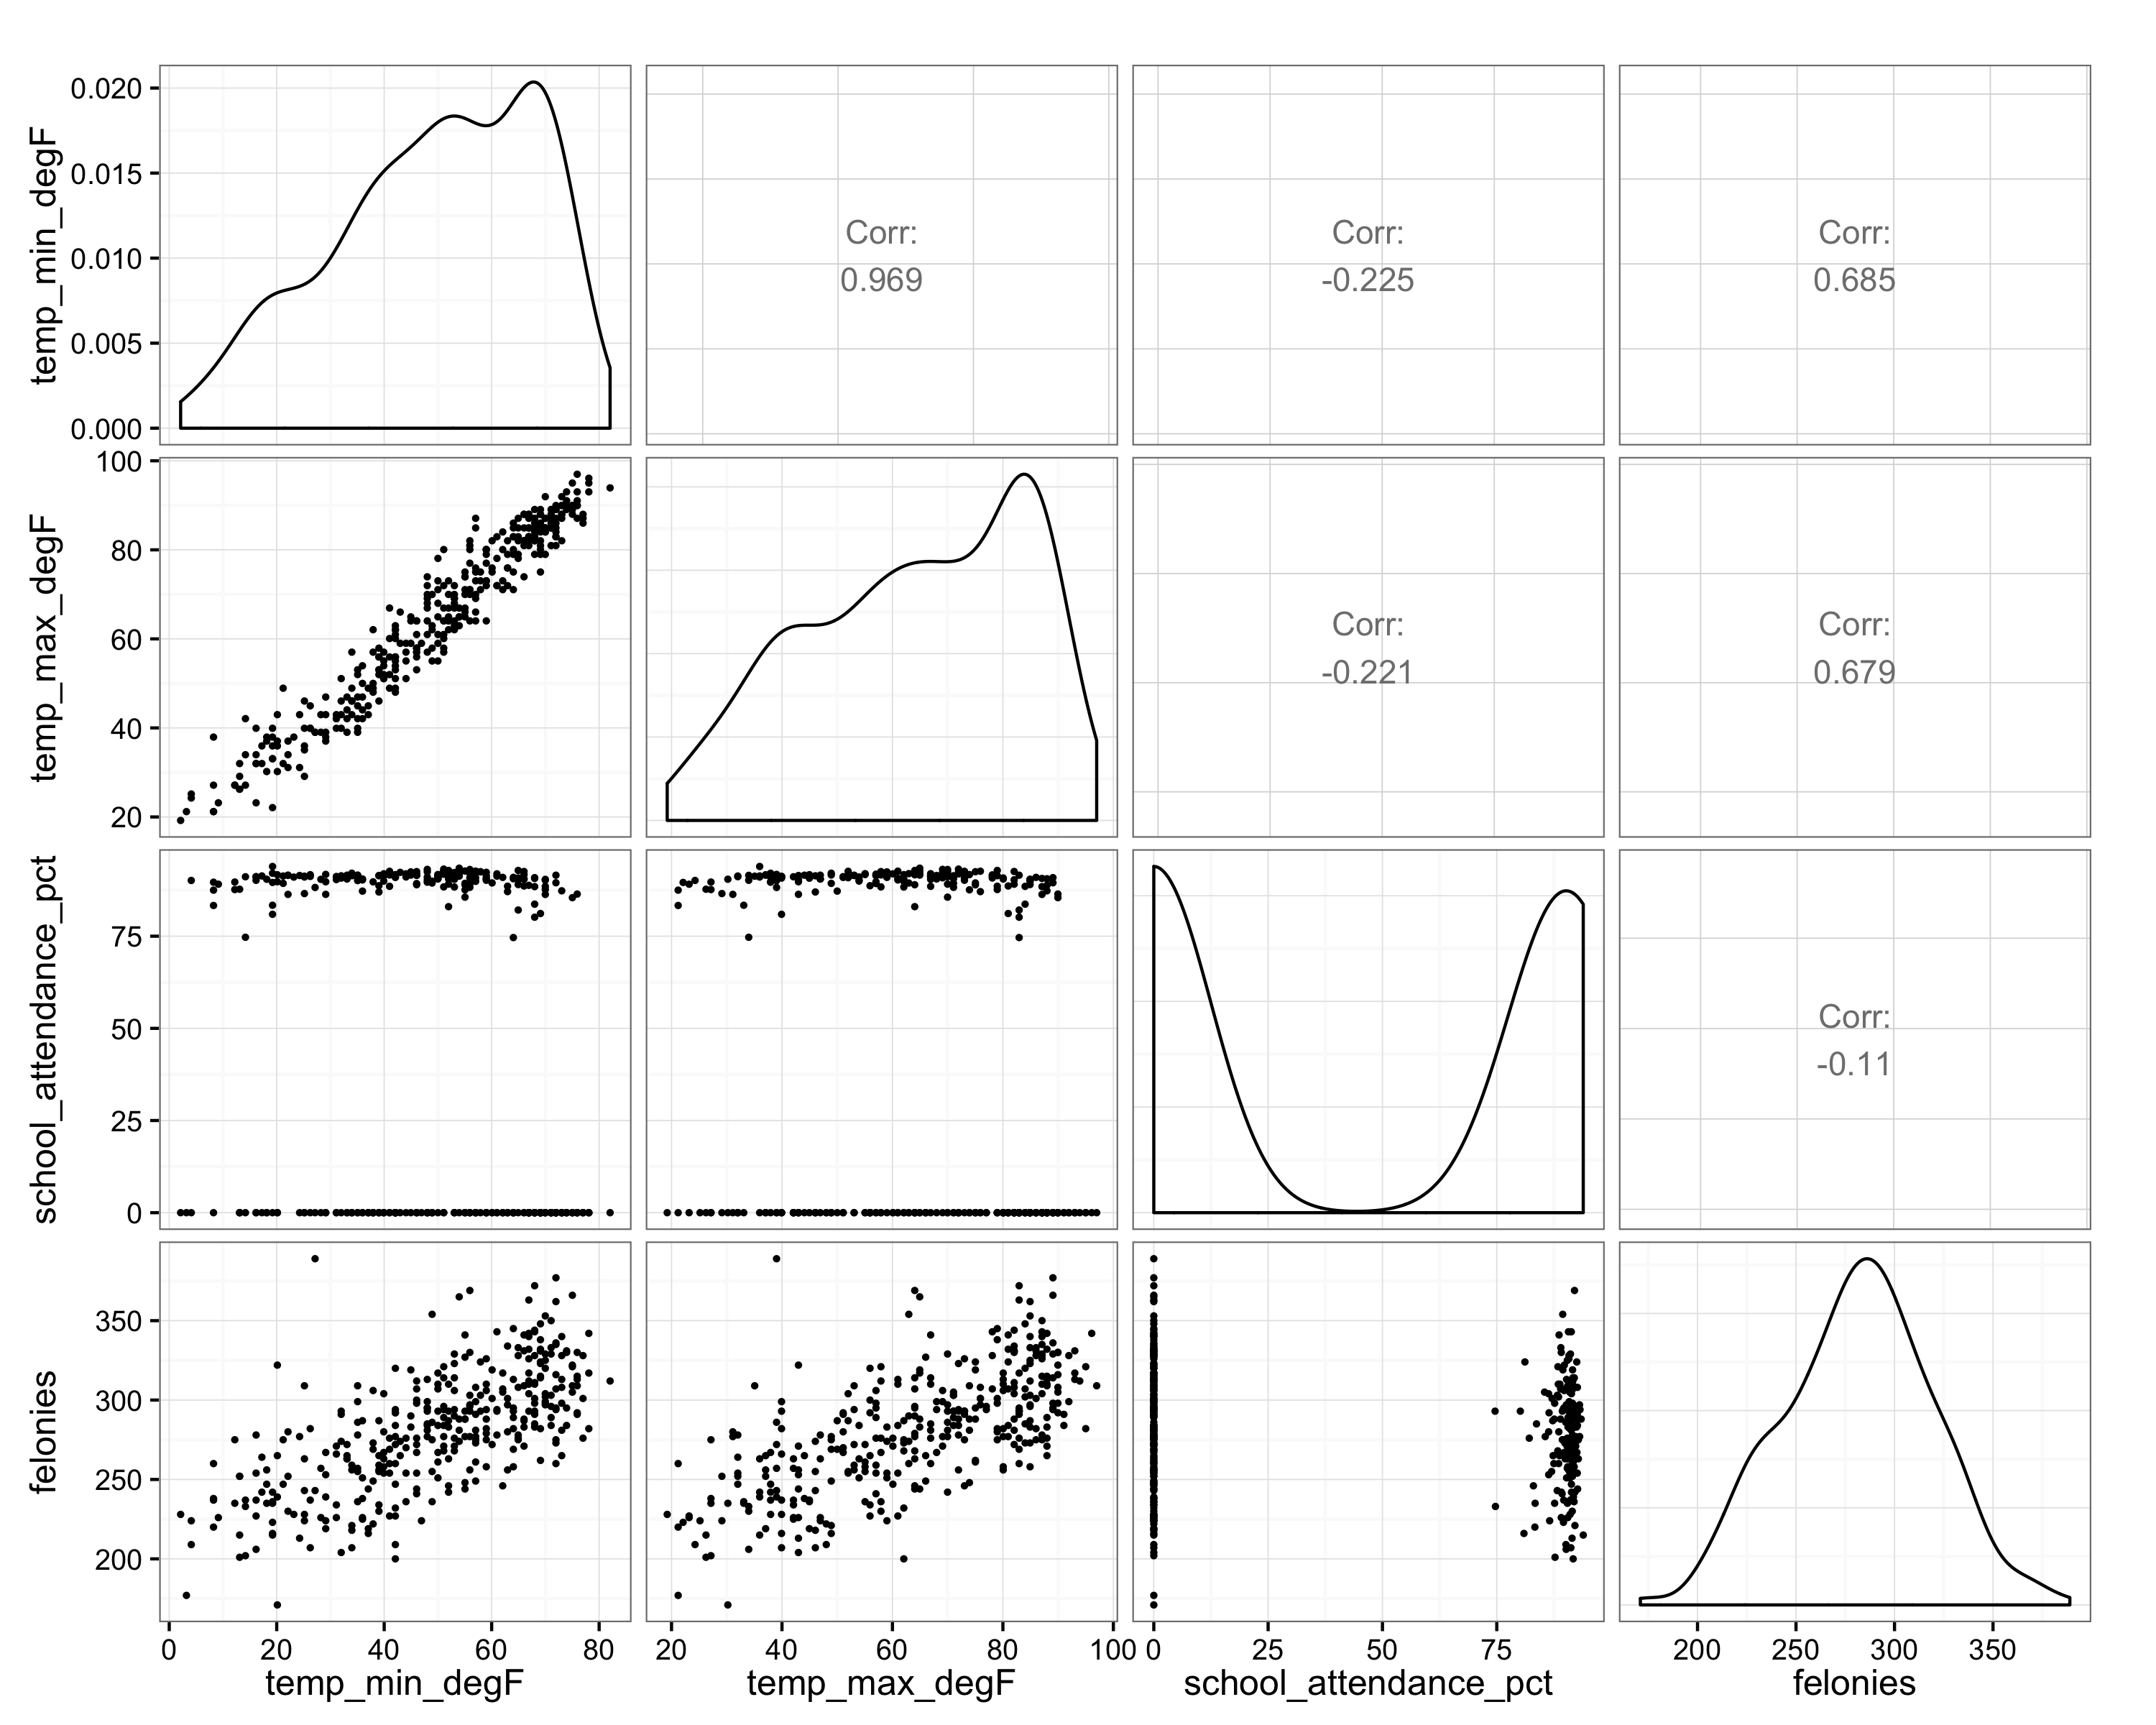
\includegraphics[width=6in]{figures/pairsNumericExclAcc.png}
	\caption{Pairwise scatterplots of some of the numeric variables in the raw dataset.}
	\label{fig:pairsNumericExclAcc}
\end{figure}


Figure \ref{fig:pairsNumericExclAcc} also shows that there is no linear relationship between \texttt{felonies} and \texttt{school_attendance_pct} (the percent of students present in school on a given day). Any non-school-day has 0\% attendance, so instead of using this as a numeric variable, we convert it to the indicator variable \texttt{is_school_day}, taking value ``1'' if NYC Public Schools were open and in session on the given date (i.e., if \texttt{school_attendance_pct} is $>0$), or value ``0'' otherwise.

Faceted boxplots of the categorical variables are shown in Figure \ref{fig:facetCategorical}.

\begin{figure}[!h]
	\centering
	\captionsetup{width=0.9\textwidth}
	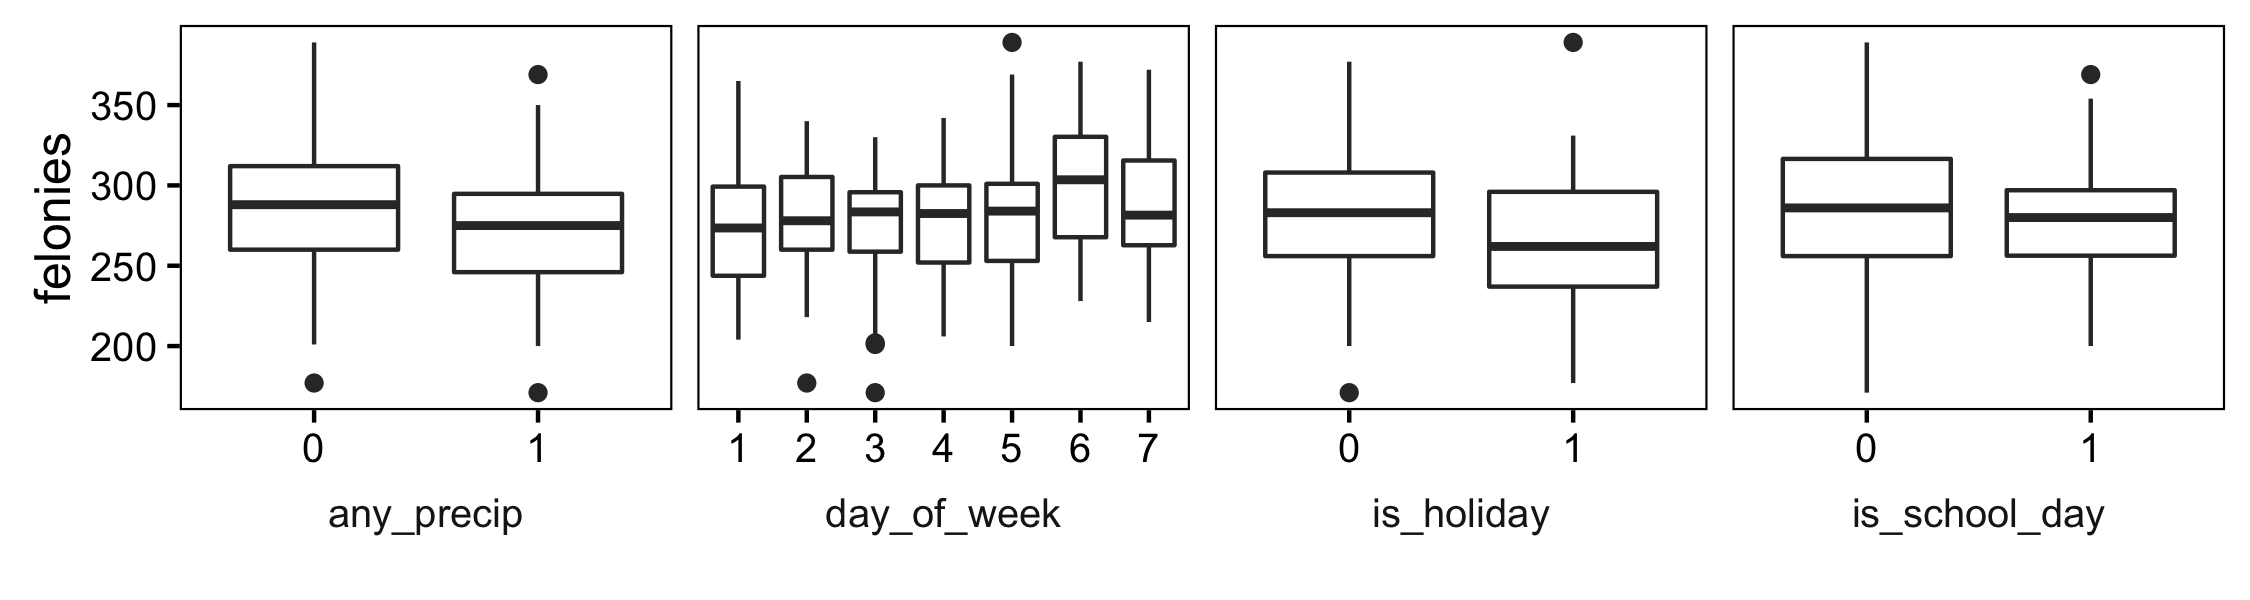
\includegraphics[width=6in]{figures/facetCategorical.png}
	\caption{Faceted boxplots of the categorical variables in the dataset.}
	\label{fig:facetCategorical}
\end{figure}

\section{Modeling the Number of Felonies Per Day}

In this section we use simple and multiple linear regression to model the number of felonies per day (the first and second questions of interest).

\subsection{Assumptions}
\label{sec:feloniesAssumptions}

We first assume that each occurrence of a felony is an independent Bernoulli event with very low probability $p$. The sum of these Bernoulli events is the number of felonies that occur on a given day. This sum follows a binomial distribution where $n$ is the number of opportunities for a felony to occur --- as a rough approximation this might be on the order of the population of NYC ($\sim 8.4$ million). Since $n$ is large enough, we can approximate this binomial distribution with a normal distribution.

We also assume the four assumptions of linear regression:
\begin{itemize}
\setlength\itemsep{-1pt}

\item Linearity: \texttt{felonies} can be expressed as linear combination of the independent variables
\item Homoscedasticity (constant variance): $\text{Var}(Y|X_1,\ldots, X_p)$ is the same at all values of $X_1,\ldots, X_p$
\item Normality: residuals of the fit are normally distributed
\item Independence: residuals of the fit are independent
\end{itemize}


\subsection{Exploratory Models}

As an exploratory step, we initially perform a simple linear regression of felonies on temperature. The regression coefficients, standard errors, and p-values are shown below: \todo{Might not even need to show these here, as long as I keep the summary in the next paragraph.}

\begin{codeSmall}
               Estimate Std. Error t value Pr(>|t|)    
(Intercept)   213.11913    4.07082   52.35   <2e-16 ***
temp_min_degF   1.38097    0.07709   17.91   <2e-16 ***
\end{codeSmall}

%Residual standard error: 27.48 on 363 degrees of freedom
%Multiple R-squared:  0.4692,	Adjusted R-squared:  0.4678 
%F-statistic: 320.9 on 1 and 363 DF,  p-value: < 2.2e-16

There is overwhelming evidence of an association between felonies and temperature. For every 1 $\degf$ increase in temperature, there are 1.38 additional felonies per day (95\% CI 1.22938 to 1.532569, two sided p-value $<2\times10^{-16}$ for a test that the coefficient is 0).

What's most interesting here, however, are the observations with high residuals, as shown in the residual plot in Figure \ref{fig:lm1Residuals}. Some days with large residuals aren't modeled well by temperature alone --- Jan. 1, 2015, for example, a federal holiday, had many more felonies than expected, given the temperature on that day. Including other covariates in the model, like \texttt{is_holiday} (an indicator as to whether the day is a NY/federal holiday), might help to account for some of this behavior. We next add these additional variables in Section \ref{sec:modelFeloniesMultipleRegression}.

\begin{figure}[!h]
	\centering
	\captionsetup{width=0.8\textwidth}
	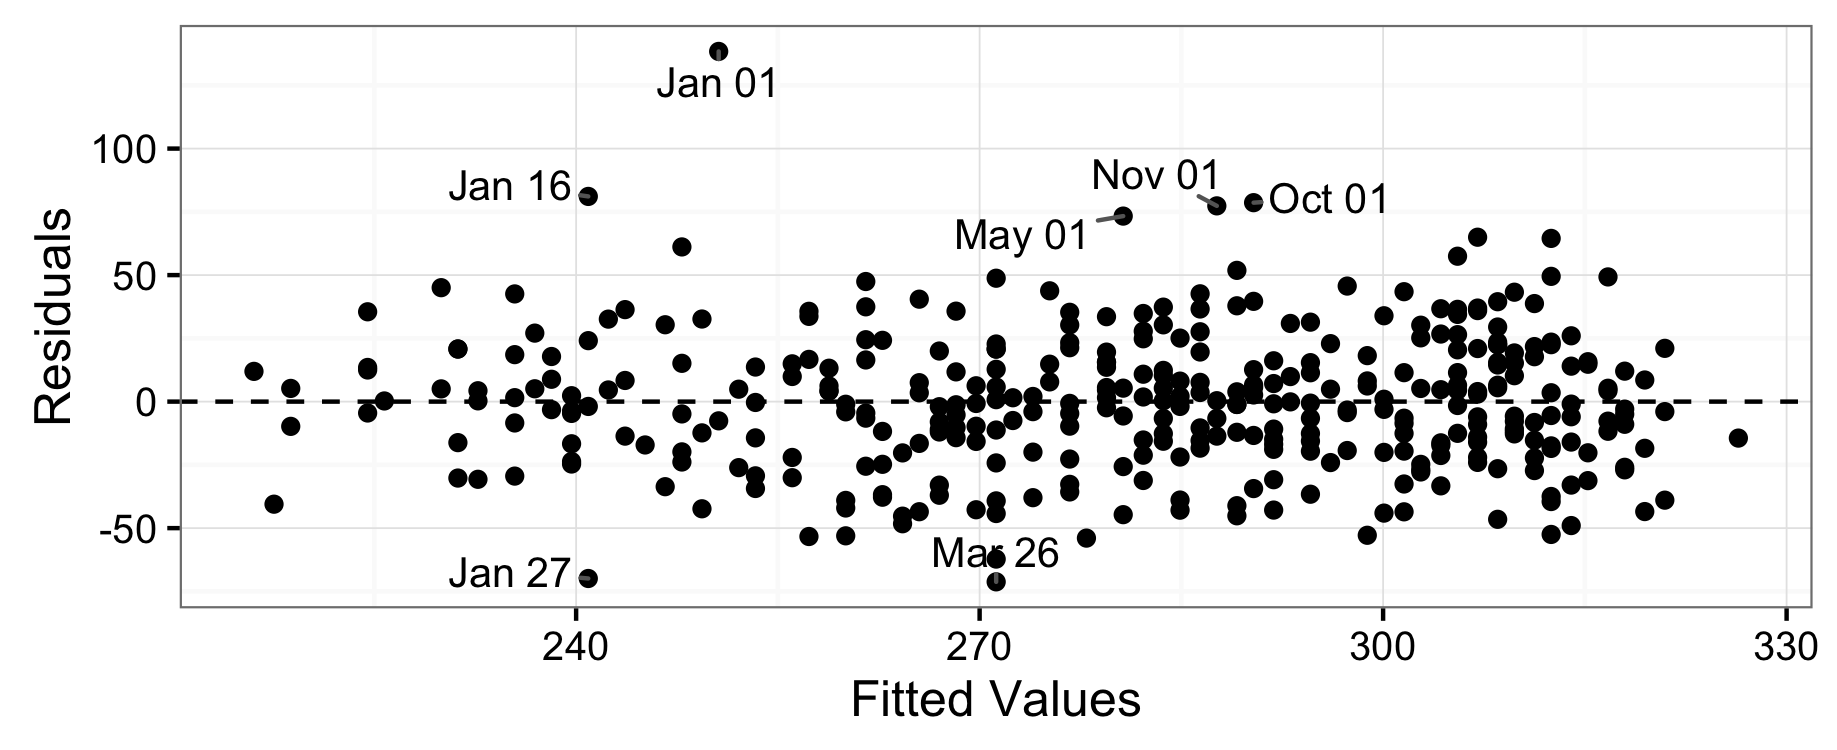
\includegraphics[width=4.25in]{figures/lm1Residuals.png}
	\caption{Residual plot for the regression of \texttt{felonies} on \texttt{temp_min_degF}.}
	\label{fig:lm1Residuals}
\end{figure}

%% two-column figure
%\begin{figure}[!h]
%  \centering
%  \captionsetup{width=0.8\textwidth}
%  \subfloat[Residual plot.]
%  		{\includegraphics[width=0.46\textwidth]
%  		{figures/lm1Residuals.png}\label{fig:lm1Residuals}}
%  \hfill
%  \subfloat[Q-Q plot.]
%  		{\includegraphics[width=0.46\textwidth]
%  		{figures/lm1QQ.png}\label{fig:f2}}
%  \caption{Residual plot and Q-Q plot for the regression of \texttt{felonies} on \texttt{temp_min_degF}.}
%\end{figure}

There are some potentially problematic observations with high leverage or large studentized residuals, but there was no change in interpretation after removing these observations from the dataset. Also note that we tested higher order terms of \texttt{temp_min_degF} in a multiple regression, but only the first-order term was significant.


\subsection{Statistical Analysis}
\label{sec:modelFeloniesMultipleRegression}

We next incorporate additional covariates, performing a multiple linear regression of felonies on the variables shown in the regression summary below:

\begin{codeSmall}
                           Estimate Std. Error t value Pr(>|t|)    
(Intercept)               210.71208    5.66649  37.186  < 2e-16 ***
temp_min_degF               1.38099    0.08768  15.750  < 2e-16 ***
any_precip1               -21.01037    8.59459  -2.445 0.014990 *  
is_holiday1                -6.00627    7.68276  -0.782 0.434865    
is_school_day1              5.94836    3.74662   1.588 0.113258    
day_of_week2                0.06874    5.73913   0.012 0.990450    
day_of_week3               -3.29691    5.70419  -0.578 0.563647    
day_of_week4               -3.46950    5.71773  -0.607 0.544376    
day_of_week5               -0.17653    5.68349  -0.031 0.975239    
day_of_week6               19.01055    5.69764   3.337 0.000938 ***
day_of_week7               14.21319    5.02454   2.829 0.004940 ** 
temp_min_degF:any_precip1   0.15666    0.16512   0.949 0.343385    
\end{codeSmall}

%Residual standard error: 25.58 on 353 degrees of freedom
%Multiple R-squared:  0.5527,	Adjusted R-squared:  0.5388 
%F-statistic: 39.66 on 11 and 353 DF,  p-value: < 2.2e-16

After accounting for temperature, there is convincing evidence that felonies is associated with precipitation. On average there are 21 fewer felonies on days with precipitation that on days without (95\% CI: 4 to 38 fewer felonies; two-sided p-value: 0.014990). The data also provides overwhelming evidence that felonies is associated with day of week (p-value $3 \times 10^{-6}$ from an extra sum of squares F-test) --- compared to Sundays, Fridays have 19 more felonies on average (95\% CI: 8 to 30 more felonies; two-sided p-value: 0.000938), and Saturdays have 14 more felonies on average (95\% CI: 4 to 24 more felonies; two-sided p-value: 0.004940).

After accounting for temperature, the holiday indicator, school day indicator, and the interaction between temperature and precipitation are not significant (two-sided p-values: 0.434865, 0.113258, and 0.343385, respectively).

\subsection{Model Checking}

To check the validity of our model, we examine a residual plot and Q-Q plot in Figure \ref{fig:lm4ResidualsQQ}. The residual plot doesn't reveal any significant violations of the linearity, constant variance, or independence assumptions, and the Q-Q plot shows that the residuals aren't perfectly normal, but that normality isn't a bad approximation.

% two-column figure
\begin{figure}[!h]
  \centering
  \captionsetup{width=0.8\textwidth}
  \subfloat%[Residual plot.]
  		{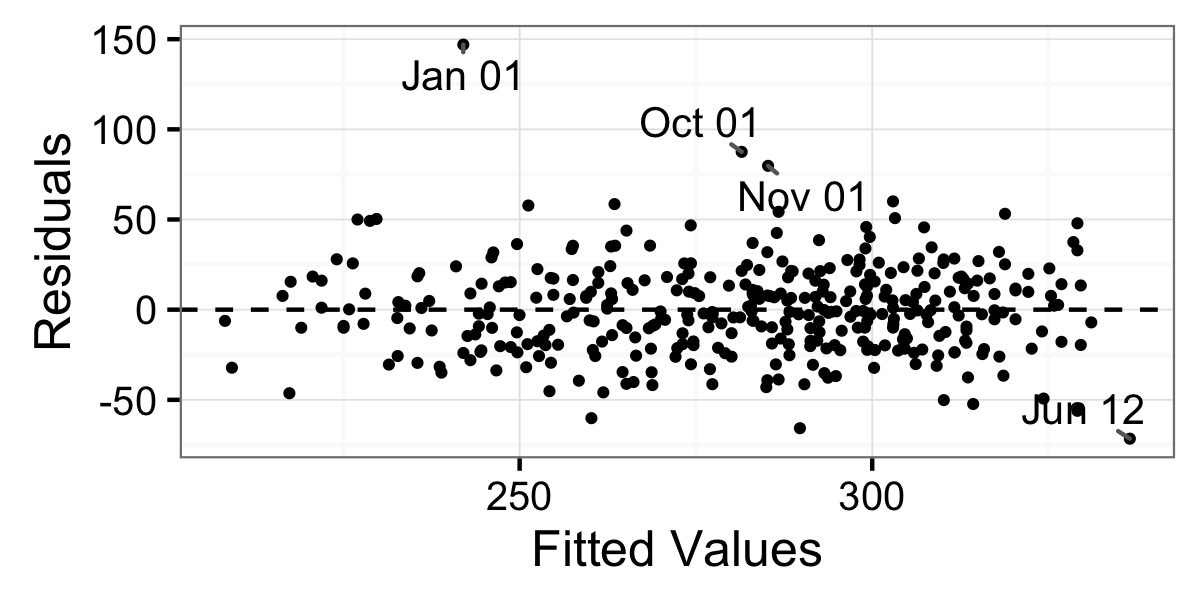
\includegraphics[width=0.46\textwidth]
  		{figures/lm4Residuals.png}\label{fig:lm4Residuals}}
  \hfill
  \subfloat%[Q-Q plot.]
  		{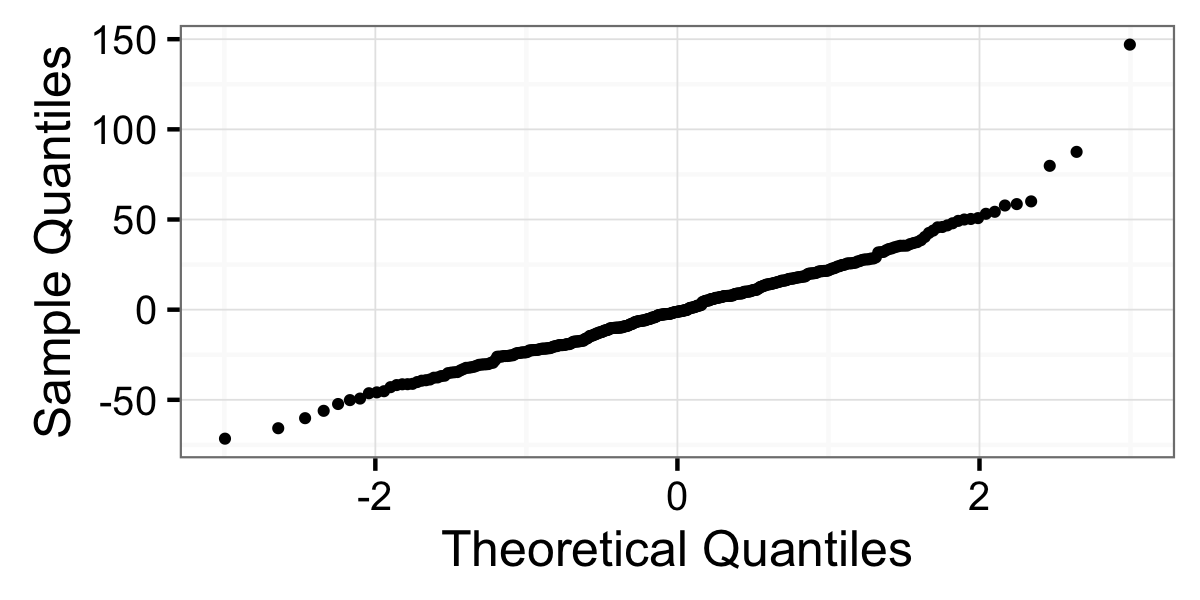
\includegraphics[width=0.46\textwidth]
  		{figures/lm4QQ.png}\label{fig:lm4QQ}}
  \caption{Residual plot and Q-Q plot for the regression of \texttt{felonies} on \texttt{temp_min_degF}, \texttt{any_precip}, \texttt{is_holiday}, \texttt{is_school_day}, \texttt{day_of_week}, and the interaction between \texttt{temp_min_degF} and \texttt{any_precip}.}
  \label{fig:lm4ResidualsQQ}
\end{figure}

Next, we check for influential observations by examining leverages, studentized residuals, and Cook's distances. From these case influence statistics there are 17 potentially problematic observations. Partial residual plots for \texttt{is_holiday} and \texttt{is_school_day} (two of the non-significant variables from the regression) are shown in Figure \ref{fig:lm4Pres}. If we exclude the 17 potentially problematic observations (coded with blue triangles in Figure \ref{fig:lm4Pres}), it appears as though holidays have fewer felonies than non-holidays, and school days tend to have more felonies than non-school days.

% two-column figure
\begin{figure}[!h]
  \centering
  \captionsetup{width=0.8\textwidth}
  \subfloat%[caption text]
  		{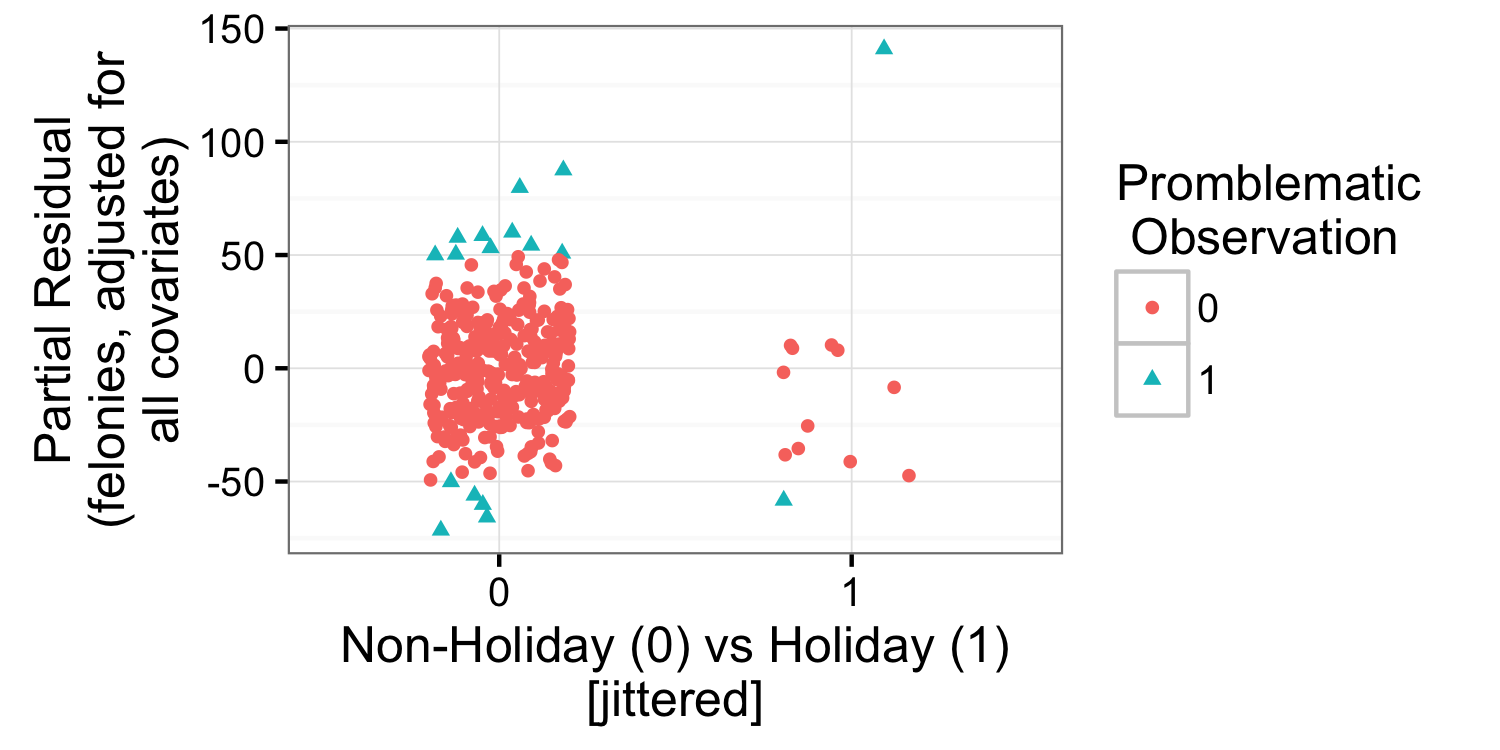
\includegraphics[width=0.5\textwidth]
  		{figures/lm4PresIsHoliday.png}\label{fig:lm4PresIsHoliday}}
  \hfill
  \subfloat%[caption text]
  		{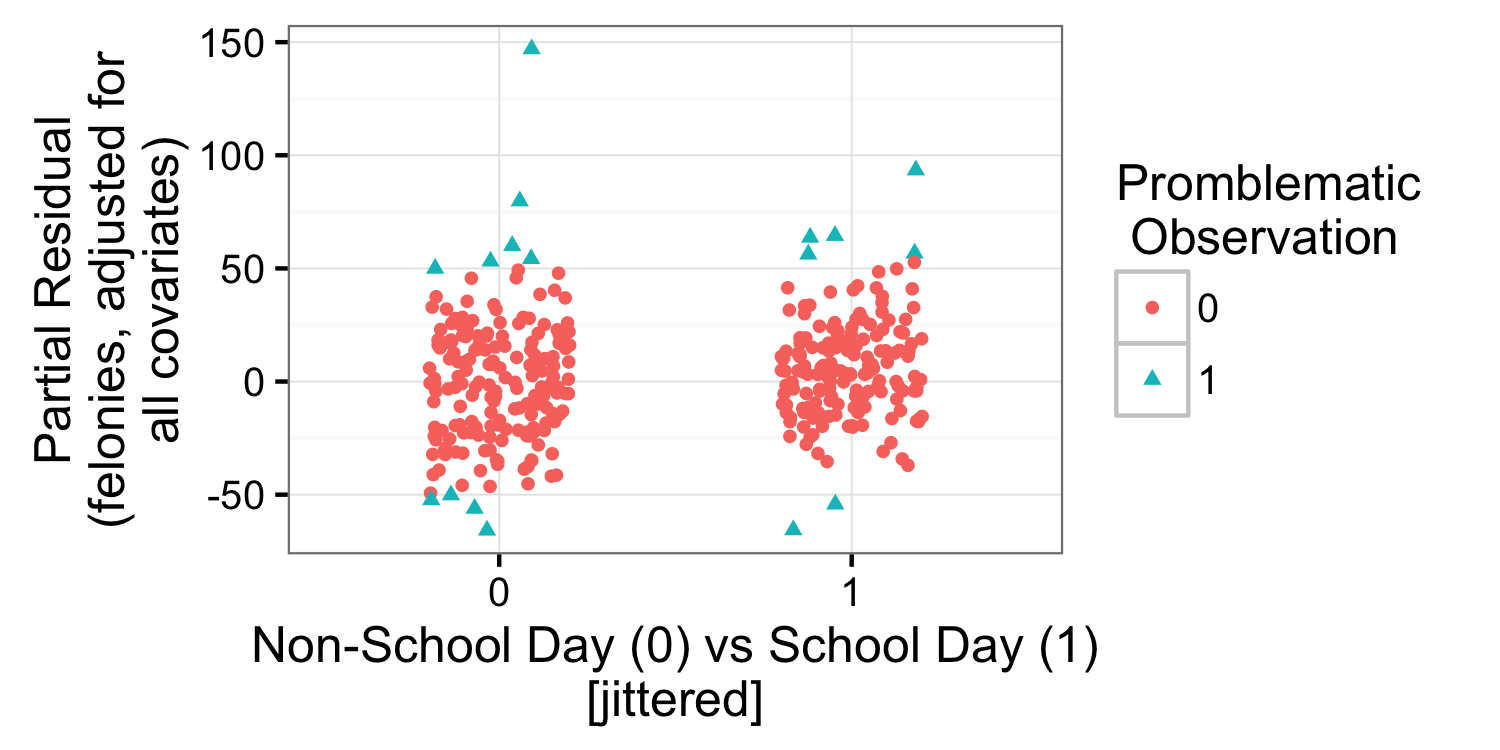
\includegraphics[width=0.5\textwidth]
  		{figures/lm4PresIsSchoolDay.png}\label{fig:lm4PresIsSchoolDay}}
  \caption{Partial residual plots for \texttt{is_holiday} and \texttt{is_school_day}. In each plot, the 17 potentially problematic observations are coded with blue triangles.}
  \label{fig:lm4Pres}
\end{figure}



\subsection{Model Improvement}

We re-fit the regression from Section \ref{sec:modelFeloniesMultipleRegression}, but now excluding the 17 potentially problematic observations. The regression coefficients are shown below:

\begin{codeSmall}
                           Estimate Std. Error t value   Pr(>|t|)    
(Intercept)               202.29838    4.72876  42.780    < 2e-16 ***
temp_min_degF               1.47704    0.07321  20.175    < 2e-16 ***
any_precip1               -20.41161    7.20033  -2.835    0.00486 ** 
is_holiday1               -13.26886    6.82627  -1.944    0.05275 .  
is_school_day1              6.69136    3.12660   2.140    0.03306 *  
day_of_week2                4.01255    4.81800   0.833    0.40553    
day_of_week3                0.10726    4.73001   0.023    0.98192    
day_of_week4               -0.18818    4.73899  -0.040    0.96835    
day_of_week5               -2.77336    4.80166  -0.578    0.56393    
day_of_week6               22.99155    4.79145   4.798 0.00000241 ***
day_of_week7               19.50039    4.21983   4.621 0.00000545 ***
temp_min_degF:any_precip1   0.13801    0.13747   1.004    0.31615    
\end{codeSmall}

%Residual standard error: 20.85 on 336 degrees of freedom
%Multiple R-squared:  0.6773,	Adjusted R-squared:  0.6667 
%F-statistic:  64.1 on 11 and 336 DF,  p-value: < 2.2e-16


After removing the 17 problematic observations, the holiday indicator and school day indicator are now significant. The interaction between temperature and precipitation still isn't significant, even after removing the 17 observations. \todo{Possibly include inferences here. Otherwise, include them in the Conclusion section.}


%If hitting the page limit, probably no need to remove the interaction term (models lm6 and lm7).




\section{Modeling the Day-to-Day Change in the Number of Felonies Per Day}

As a supplementary analysis, we now explore if changes in the number of felonies, as compared to the previous day, is associated with large increases in temperature, after taking our other covariates into account (the third question of interest). The theory here is that spikes in temperature (e.g., at the beginning of a heat wave or on the first few days of spring) might influence the number of felonies that occur. In this section, \texttt{temp_jump} indicates if the temperature has increased by more than $8\degf$ as compared to the previous day.




\subsection{Assumptions}

In this section we use multiple linear regression to model \texttt{felonies_diff} (the difference in the number of felonies as compared to the previous day; see Section \ref{sec:dataset}). Again we assume the 4 assumptions of linear regression, as outlined in Section \ref{sec:feloniesAssumptions}.

\subsection{Statistical Analysis}

We now perform a multiple linear regression of \texttt{felonies_diff} on the variables shown in the regression summary below:

\begin{codeSmall}
                          Estimate Std. Error t value Pr(>|t|)    
(Intercept)              -19.09877    6.66217  -2.867 0.004397 ** 
temp_jump1                21.73759   16.38144   1.327 0.185381    
temp_min_degF              0.12321    0.09743   1.265 0.206821    
any_precip1               -1.90533    3.72032  -0.512 0.608873    
is_holiday1                0.95049    9.39575   0.101 0.919480    
is_school_day1             6.95124    4.60154   1.511 0.131779    
day_of_week2              12.22189    6.99960   1.746 0.081669 .  
day_of_week3               2.91295    6.97539   0.418 0.676491    
day_of_week4              11.05330    6.99797   1.580 0.115120    
day_of_week5               9.94665    6.94328   1.433 0.152872    
day_of_week6              25.59847    6.96531   3.675 0.000275 ***
day_of_week7               1.79654    6.14494   0.292 0.770183    
temp_jump1:temp_min_degF  -0.28253    0.34895  -0.810 0.418679    
\end{codeSmall}

%Residual standard error: 31.23 on 352 degrees of freedom
%Multiple R-squared:  0.103,	Adjusted R-squared:  0.07247 
%F-statistic:  3.37 on 12 and 352 DF,  p-value: 0.0001127



After accounting for temperature, precipitation, holidays, school days, and day of week, the data provides no evidence that changes in the number of felonies is associated with large increases in temperature (two-sided p-value 0.185381). The interaction between temperature and the temperature jump indicator is also not significant (two-sided p-value 0.418679).

The data provides overwhelming evidence that \texttt{felonies_diff} is associated with \texttt{day_of_week} (p-value 0.003788 from an extra sum of squares F-test) --- on Fridays, for example, there are on average 26 more felonies than on the preceding Thursday (95\% CI 12 to 39 more felonies; two-sided p-value 0.000275).


\subsection{Model Checking and Improvement}

Neither a residual plot nor a Q-Q plot (not shown) reveal any significant violations of our assumptions. Case influence statistics reveal 12 potentially influential observations, but there is no change in interpretation once they're removed.

To simplify the model, we now iteratively remove the non-significant variables from the regression, and end up with a model in which only \texttt{temp_jump} and \texttt{day_of_week} are remaining. The regression summary is shown below:

\begin{codeSmall}
             Estimate Std. Error t value Pr(>|t|)    
             Estimate Std. Error t value Pr(>|t|)    
(Intercept)   -13.338      4.383  -3.043  0.00252 ** 
temp_jump1      8.942      5.423   1.649  0.10006    
day_of_week2   16.480      6.113   2.696  0.00736 ** 
day_of_week3    6.999      6.113   1.145  0.25305    
day_of_week4   16.152      6.116   2.641  0.00863 ** 
day_of_week5   14.496      6.085   2.382  0.01773 *  
day_of_week6   30.208      6.121   4.936 1.23e-06 ***
day_of_week7    1.746      6.127   0.285  0.77589    
\end{codeSmall}

%Residual standard error: 31.17 on 357 degrees of freedom
%Multiple R-squared:  0.0941,	Adjusted R-squared:  0.07634 
%F-statistic: 5.298 on 7 and 357 DF,  p-value: 8.909e-06

The temperature jump indicator still is not significant (two-sided p-value 0.10006). Only the \texttt{day_of_week} variable has a significant relationship with day-to-day changes in the number of felonies (p-value $9 \times 10^{-6}$ from an extra sum of squares F-test) --- Fridays, for example, generally have 30 more felonies than the preceding Thursday (95\% CI 18 to 42 more felonies; two-sided p-value $1 \times 10^{-6}$).


\section{Conclusions}
\label{sec:conclusion}

\subsection{Statistical Conclusions}

The data provides overwhelming evidence that felonies is associated with temperature. For every 1 $\degf$ increase in temperature, there are, on average, 1.38 additional felonies per day (95\% CI 1.22938 to 1.532569, two sided p-value $<2\times10^{-16}$).

After accounting for temperature, there is convincing evidence that felonies is associated with precipitation. On average there are 21 fewer felonies on days with precipitation that on days without (95\% CI: 4 to 38 fewer felonies; two-sided p-value: 0.014990). The data also provides overwhelming evidence that felonies is associated with day of week (p-value $3 \times 10^{-6}$ from an extra sum of squares F-test).

Initially, it did not appear that the number of felonies was associated with holidays or with school days, but after removing 17 observations with high studentized residuals, these variables became significant. From the revised model, there is suggestive, but inconclusive evidence that felonies is associated with holidays --- on average, holidays have 13 fewer felonies than non-holidays (95\% CI 0 to 27 fewer felonies; two-sided p-value 0.05275). Again from the revised model, there is moderate evidence that felonies is associated with school days --- on average, school days have 7 more felonies that non-school days (95\% CI 1 to 13 more felonies; two-sided p-value 0.03306).

In both the initial and revised models, the interaction between temperature and precipitation was not significant (two-sided p-value was $>0.3$ in both models).


From a supplementary analysis, after accounting for day of week, the data provides no evidence that day-to-day changes in the number of felonies is associated with large increases in temperature (an increase of $>8 \degf$ as compared to the previous day) (two-sided p-value 0.10006).


\subsection{Scope of Inference}

This is purely observational data --- observations weren't randomly sampled --- so these statistical associations cannot be used to draw causal connections. Further, any generalization of these results to cities other than NYC for time periods other than 2015 is speculative.



\listoftodos

\pagebreak

% To compile the bibliography: BibTeX, PDFLaTeX, Quick Build.
%\nocite{*} % This command includes all sources to be listed in the bibliography, even if uncited in the article.
%\singlespacing
%\bibliographystyle{unsrt}
%\bibliography{bib_name}

\end{document}

